\documentclass[a4paper,twoside,11pt]{article}
\usepackage[utf8]{inputenc}
\usepackage[portuguese]{babel}
\usepackage{graphicx}
\usepackage{url}
\usepackage{titlesec}


% Redefinição das margens das páginas
\setlength{\textheight}{24.00cm}
\setlength{\textwidth}{15.50cm}
\setlength{\topmargin}{0.35cm}
\setlength{\headheight}{0cm}
\setlength{\headsep}{0cm}
\setlength{\oddsidemargin}{0.25cm}
\setlength{\evensidemargin}{0.25cm}
\setlength{\parindent}{0pt}

\begin{document}

\vspace{-15mm}
\begin{figure}[h]
\begin{center}
\resizebox{80mm}{!}{
\includegraphics{logoISEL.png}}
\end{center}
\end{figure}
\vspace{-8mm}

% Title Section
\begin{center}
    \LARGE \textbf{LiftDrop} \\ % Bold title
    \LARGE Mobile App for Deliveries \\ % Subtitle in normal weight
    \vspace{8mm}
    \large Gonçalo Morais, n.º 49502, e-mail: a49502@alunos.isel.pt, tel.: 927468061 \\
    \vspace{1mm}
    \large João Ramos, n.º 49424, e-mail: a49424@alunos.isel.pt, tel.: 919222551 \\
    \vspace{5mm}
    \large \textbf{Orientador:} Miguel Gamboa, e-mail: miguel.gamboa@isel.pt \\
    \vspace{3mm}
    \large \textbf{Co-Orientador:} Diogo Silva, e-mail: diogo.silva@lyzer.tech \\
    \vspace{5mm}
    \textbf{Março de 2025}
\end{center}

\vspace{10mm}

{\sffamily
\section*{Introduction}

\vspace{5mm}

\subsection*{Contextualization}

\vspace{3mm}

The rise of the \textbf{gig economy} has transformed various industries, particularly in the food delivery sector. This economic model is characterized by short-term, flexible work arrangements where individuals take on temporary jobs, often facilitated through digital platforms. Companies such as \textbf{Uber Eats, Glovo, and Bolt Food} have leveraged this framework to revolutionize urban logistics, enabling customers to order food on demand while providing couriers with independent work opportunities.

\vspace{5mm}

By prioritizing \textbf{customer convenience}, these platforms have successfully streamlined food delivery processes through real-time technology, ensuring efficiency and reliability at scale. However, as demand for delivery services continues to grow, the gig economy also presents operational challenges, particularly affecting the couriers who sustain this system.

\newpage

\subsection*{Project Goals}

This project aims to develop a delivery-focused Android mobile application that assists couriers in efficiently handling deliveries while ensuring a seamless and informed working experience. To support the app’s functionality, we'll be implementing two separate web APIs:

\begin{itemize}
    \item \textbf{Courier API} -  A backend service that powers the mobile app, handling real-time courier updates, order assignments, and safety features.
    \item \textbf{Client Simulation API} - A backend service designed to simulate client orders.
\end{itemize}

By leveraging this architecture, we will enhance the delivery experience through the following key objectives:

\begin{itemize}
    \item \textbf{Real-time demand insights} - Using heat maps to highlight high-order density areas, helping couriers make informed decisions.
    \item \textbf{Courier safety measures} - Implementing a neighborhood safety rating system to alert couriers about high-risk locations.
    \item \textbf{Optimized order assignment} - Assigning orders efficiently based on proximity, fairness, and traffic conditions.
    \item \textbf{(Optional) Earnings tracking} - Providing insights into income and performance trends.
\end{itemize}

\section*{Scope}

Developing a mobile application focused on delivery presents challenges, particularly in real-time data handling and order assignment. Since multiple couriers interact with the platform simultaneously, the system must manage updates effectively while ensuring a smooth user experience. After some research and consideration, we identified two primary approaches to handling real-time updates and concurrency:

\begin{itemize}
    \item \textbf{Polling-based Request-Response Model} – The client periodically requests updates from the server. While simple to implement, this approach results in unnecessary network requests, increased server load, and delayed updates.
    \item \textbf{WebSockets} – A bidirectional communication protocol that allows both the client and server to send messages dynamically. While WebSockets are ideal for interactive, two-way communication (e.g., chat applications), SSE offers a simpler and more reliable approach for our needs, focusing on server-driven updates.
    \item \textbf{Event-Driven Server-Sent Events (SSE)} – The server pushes updates to clients as they occur, enabling real-time communication without the inefficiencies of constant polling. This is well-suited for unidirectional data flow (server-to-client updates).
\end{itemize}

Given the requirements of this project, we chose SSE as the preferred method for real-time updates due to its simplicity, maintainability, and efficient handling of one-way event streams. To implement SSE on Android, we will use OkHttp since Android lacks native SSE support.

\vspace{2mm}

For order assignment, the platform will consider factors like \textbf{Proximity-based allocation}, \textbf{Fair distribution}, and \textbf{Traffic-aware routing}. An external geospatial API will handle location-based calculations (distance, routing, and traffic), simplifying the implementation by reducing the need for complex in-house geospatial logic.

\vspace{2mm}

Several geospatial APIs can provide direct distance calculations between a courier and a pickup location. We chose the \textbf{Google Maps API} as it offers the most suitable free plan for the required functionalities.

\vspace{2mm}

To enhance safety, the platform will feature \textbf{neighborhood safety ratings} based on feedback from couriers who have completed deliveries in those areas. Only couriers can submit ratings, ensuring assessments reflect real delivery conditions.  

Couriers will receive alerts for high-risk areas, and \textbf{nighttime safety measures} will highlight risk-prone locations for late-night deliveries.

\section*{Architecture and Tech Stack}

The system architecture will consist of the following components:

\begin{itemize}
    \item \textbf{Application for Android}: Implemented using Jetpack Compose. The app is planned for deployment on the Google Play Store.
    \item \textbf{Backend}: Developed using Kotlin with Spring MVC, handling business logic, real-time interactions, and data management. Initially deployed using Docker on Render.
    \item \textbf{PostgreSQL Database}: Stores connections between entities along with additional order and user-related data.
\end{itemize}

The chosen tech stack was selected to meet the needs of a \textbf{courier-focused delivery app}. \textbf{Jetpack Compose} simplifies Android development with a modern UI framework, while \textbf{Kotlin with Spring MVC} ensures a structured and maintainable backend for handling RESTful services and real-time updates.  

\vspace{2mm}

\textbf{PostgreSQL} was chosen for its \textbf{geospatial query support}, enabling efficient location-based order assignments. The backend is containerized with \textbf{Docker} and deployed on \textbf{Render} to facilitate \textbf{scalability and cloud-based deployment}.  

\subsection*{Challenges Ahead}

Although our project aims to improve the courier experience through innovative features, several challenges must be addressed during development and deployment.

\begin{itemize}
\item \textbf{Real-Time Data Synchronization}: Ensure consistent and reliable updates between couriers, the server, and the application without compromising performance or data integrity.

\item \textbf{Scalability}: As the user base grows, maintain system performance and responsiveness while scaling up server resources and database capabilities.

\item \textbf{User Interface Design}: Design an intuitive and efficient user interface using Jetpack Compose that meets the diverse needs of both couriers and administrators.

\item \textbf{Integration Complexity}: Integrating third-party APIs for geospatial data and safety ratings while maintaining system stability and reliability.

\item \textbf{Testing and Validation}: Rigorously testing the application using automatic tests.
\end{itemize}

Addressing these challenges proactively will be crucial to delivering a robust and effective mobile application that meets the demands of both couriers and users alike.

\section*{Features}

The \textbf{LiftDrop} mobile app is designed to enhance the delivery experience for couriers by providing a seamless, real-time, and secure workflow. The key features of the app include:

\begin{itemize}
    \item \textbf{Safety and Security}
    \begin{itemize}
        \item \textbf{Neighborhood Safety Ratings}: Allows couriers to rate delivery areas based on their experiences, helping others avoid high-risk zones.
        \item \textbf{Risk Alerts}: Sends notifications warning couriers about potentially unsafe locations.
        \item \textbf{Nighttime Safety Measures}: Provides additional safety insights for late-night deliveries.
    \end{itemize}

    \item \textbf{Courier Performance Insights}
    \begin{itemize}
        \item \textbf{Earnings Tracking}: Displays detailed breakdowns of income over time.
        \item \textbf{Delivery Statistics}: Provides performance trends to help couriers optimize their workflow.
    \end{itemize}

    \item \textbf{Real-Time Demand Insights}
    \begin{itemize}
        \item \textbf{Heatmaps}: Displays visual indicators highlighting high-order density areas, helping couriers position themselves more effectively.
    \end{itemize}
\end{itemize}

}

\section*{Project Plan}

\begin{figure}[h]
    \centering
    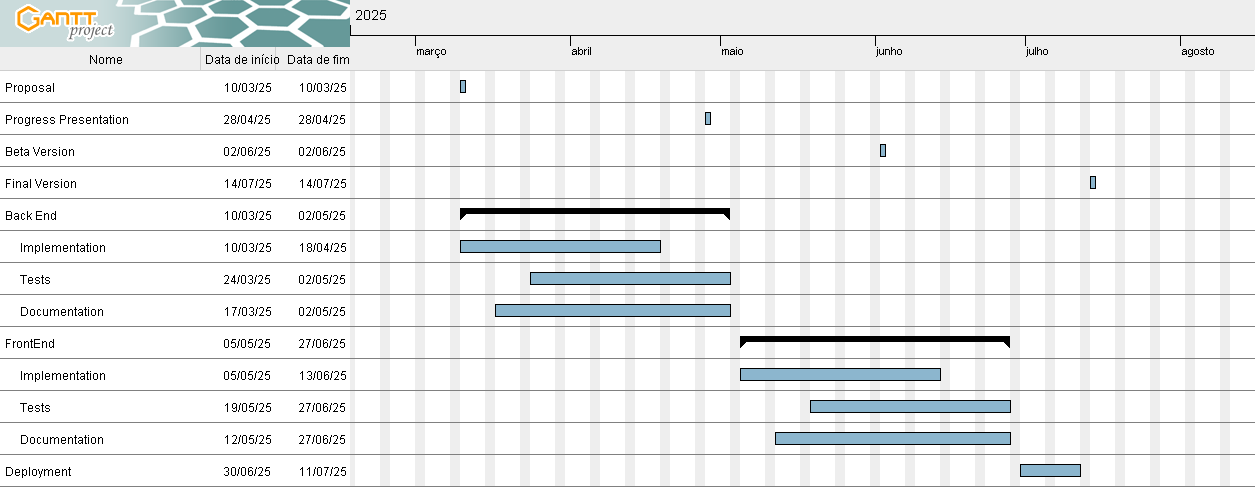
\includegraphics[width=\textwidth]{ProjectPlan.png}
    \caption{Project Plan}
    \label{fig:project-plan}
\end{figure}

\bibliographystyle{alpha}
\bibliography{sample}

\end{document}